\documentclass[11pt,a4paper,fleqn,twoside]{article}
% Uncomment the following line to allow the usage of graphics (.png, .jpg)
\usepackage[pdftex]{graphicx}
\usepackage[a4paper,inner=2.2cm,outer=2.2cm,bottom=2.2cm,headheight=1cm]{geometry} % to change the page dimensions
% Comment the following line to NOT allow the usage of umlauts
\usepackage[utf8]{inputenc}
\usepackage[T1]{fontenc}
\usepackage{hyperref}

\usepackage{titling}
\renewcommand{\droptitle}{50pt}

\pretitle{%
  \begin{center}
  \LARGE
  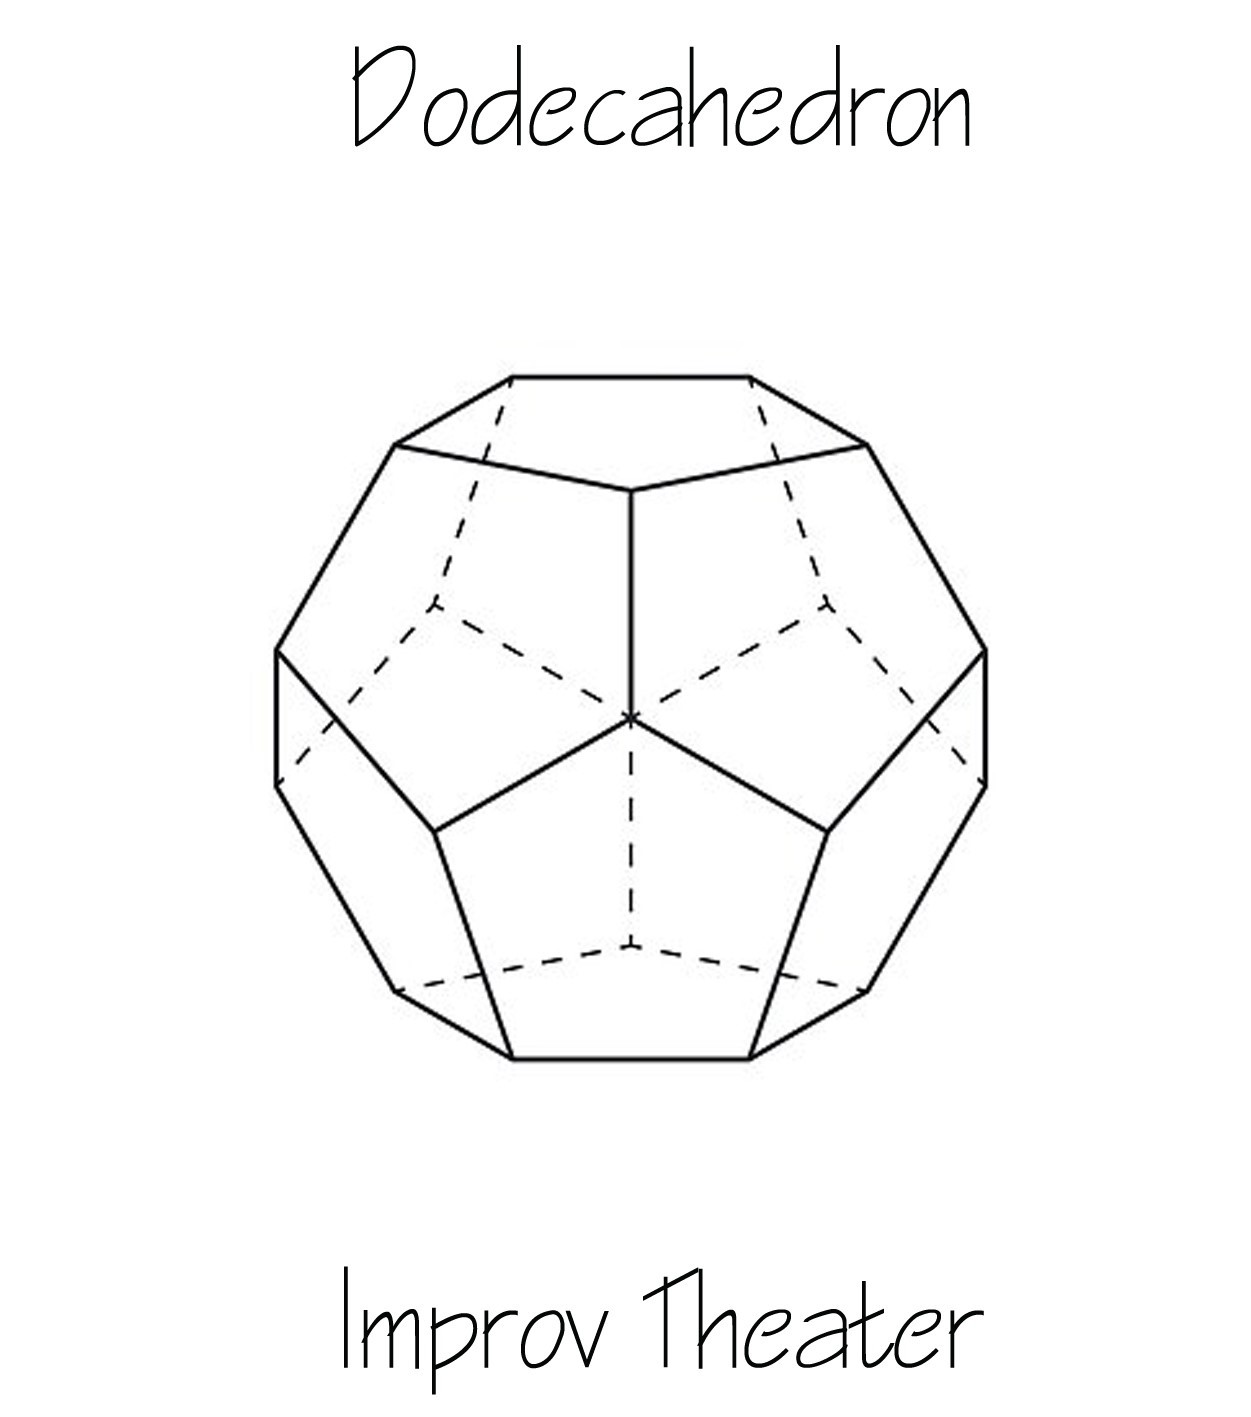
\includegraphics[width=0.6 \textwidth]{logo}\\[\bigskipamount]
}
\posttitle{\end{center}}
\title{Diary for a new theater group}
\author{Dodecahedron Improv Group}

\begin{document}
\maketitle
\clearpage
\tableofcontents
%%%%%%%%%%%%%%%%%%%%%%%%%%%%
% Sections
\clearpage

\section{Introduction}

We are the Dodecahedron Improv Theater (DIT) group, a non-profit group of students and young professionals from different paths of life who gather on a weekly basis to learn and rehearse theater improvisation. Our group was brought to life in July 2017. We meet on weekly basis for rehearsals at ETH Zürich zentrum, usually on Wednesdays. One can find more updated information about us in our \href{https://www.facebook.com/dodecahedronimprovtheater/}{Facebook page}.

\subsection{Improvisational theater, Improv}

The improvisational theater or, also called ``Improv'' is just another form of theater. It just have the particularity that there is not predefined script of the story that it is going to be performed on the stage. Instead, it will be the actors of improvisers the ones in charge of creating it, on the go. In Improv the people on the stage are the actors, producers and directors of the ongoing plot, everything at the same time.

Their stories will usually be motivated by some external interaction. In occasions the audience will provide some aspect of the story to be told that will guide the improvisers, for example a relationship between characters, the place will the action will take place or a general idea that shall be translated into a plot. 

\section{Sessions diary}

\subsection{Wednesday 27th March}

We worked on these topics, which are later described in more detail.
%
\begin{itemize}
  \item Storytelling
  %
  \item Be obvious, not original
  %
  \item Status
\end{itemize}

\subsubsection{Storytelling}

This concept refers to the ability of the improviser to tell a story that is well understood and accepted by the audience. Actors who are used to act on script-based theater plays struggle with this, since they are used to need to worry about this part of the play. Instead, they can focus on the character creation and its projection on the stage. However, the improvisers needs to embrace this opportunity to create a story on the fly. He needs to be able to take the audience by the hand and guide them through his/her imagination. This ride needs to be a gentle ride for the audience, otherwise they will lose the interest and disconnect from the improviser. A basic story is made of the following phases: \begin{center}Flat-land $\Longrightarrow$ Turbulent-land $\Longrightarrow$ Arrival-land. \end{center} Initially, the story will start in the ``Flat-land'', where everything is settle up. The characters are introduced, their reciprocal relationship is presented and the space where the action takes place is drawn. Everything is plain in ``Flat-land'', no catchy adventure is introduced, so the audience has really any reason to care about what it is going to come.
%
At this point, the story may jump into the ``Turbulent-land'' where the event that interrupt the initial setting of ``Flat-land'' is introduced. Now the objective is to provide the audience with a reason to care and to be interested. During the ``Turbulent-land'', the characters react to the new situation and they might do it while playing low or high. There might be drama or comedy.
%
Finally, the issue previously presented during the ``Turbulent-land'' needs to be resolved during the ``Arrival-land''. After the issue being resolved, a new flat-like situation if shown before the story ends. This may be the same or different from the one presented during the ``Flat-land''.

\subsubsection{Status}

We continued working on this topic. Status is power, dynamic power. Status is something that the characters have, show and influence. Every little of their actions has an attribute related to the power that the action shows, or the power that it is exchanged as a result of its execution. Some people in the group need to work a little bit more in the status roles when they do not feel very comfortable. Specific people that require to improve their capacity to adapt their status are:
%
\begin{itemize}
  \item Aurora needs to learn how to get angry and play high status. She tends to play low status and avoid conflict. This behavior is inherit to her way of being. She can use Improv to explore this other side of herself. 
  \item Paschalis needs to improve how to play low status. He cannot remove the naughty smile of his face when he is trying to play low. We need to force him to play low.
\end{itemize}

\subsubsection{Be obvious, not original}

The objective is to show people how to manage the expectations of the audience. Everything that appears in the stage has to be at the same time expected and unexpected by the audience. Otherwise, they will disconnect from the improviser who is presenting the story. The proper improv concept is ``Shelving and Reincorporating''. The first terms refers to the act of placing items of the story in an imaginary shelf which is the memory of the audience, while the second refers to the act of later picking these items up to bring them into the story . The audience will then understand that, because the object was previously introduced, any action or new story situation that may be derived from it, is plausible and obvious at the same time. For instance, if I introduce in my story that my character is a fan of Michael Jackson and today is the anniversary of his death; then it may make sense that, later in the story, the real Michael Jackson materializes himself in the middle of my living room. 

\subsubsection{For the next session}

\noindent
Some ideas for the next session are the following:

\begin{itemize}
  \item Keep working on the status. Focus on the people who required to improve their relationship with the status.
  \item Repeat on the ``pedo-culo-caca-pis'' concept
\end{itemize}

\end{document}